\documentclass[../book-template.tex]{subfiles}

\begin{document}

\chapter{Dictionary Learning}
In the last chapter, we talked about finding better representation for data in terms of sparsity, where for a signal its representation can be in a high dimensional space but with only a few entries non-zero. In this chapter, we will explore the following idea: instead of manually choosing bases like wavelets or Fourier basis, can we somehow learn a good dictionary based on some given data? Our discussion will start with a brief introduction to Compressive sensing, which as mentioned in section \ref{sec_9_comp_sens} belongs to this context of sparseness. We will then talk about how to conduct dictionary learning in terms of matrix factorization, specifically with K-SVD algorithm.
\section{Compressive Sensing}
Recall our assumption that many types of signal/data are sparse in certain basis. What we have done in the last chapter is to transform such signals with proper ${\bf U}$, and then we can efficiently transmit data in their sparse coding given both the sender and receiver having the same dictionary. This means that when we take a picture, our camera first measure all the pixels, but after an appropriate change of basis we ``throw away'' most of them. This sounds rather wasteful. The natural question raises is: if only a few degree of freedom are needed for representing the data, why not measuring the data in a more efficient way, where we take considerably less measurements than the number of pixels. 
\par This idea is really at the heart of compressive sensing, and it is of great importance in the sense that it decreases acquisition time, power assumption and required storage. For an example, think about photoshooting in space. It saves memory and battery power if fewer measurements is required for taking a picture. For another important application for compressive sensing, high-resolution MRI images require patients to be perfectly still during the scanning. Decreasing the number of measurements with compressive sensing can significantly reduce the scanning time saving the energy consumption and causing less damage to the patients.
\par To build the concept, consider the original signal denoted by ${\bf x}\in \mathbb{R}^D$ which is $K$-sparse in orthonormal basis ${\bf U}\in\mathbb{R}^{D\times D}$:
\begin{equation*}
	{\bf x}={\bf Uz},\quad {\rm s.t.}\quad \|{\bf z}\|_0=K.
\end{equation*}
The idea is to acquire set ${\bf y}$ of $M$ linear combinations of the signal, like instead of measuring all pixels in an image, we somehow only compute a few linear combinations of all pixels, and hopefully these measurements (linear features) can be used to reconstruct the original signal. Formally, we have
\begin{align*}
	&y_k=\langle {\bf w}_k,{\bf x}\rangle,\quad k=1,\dots,M\\
	&{\bf y}={\bf Wx}={\bf WUz}=:{\bf \Theta z},\ {\rm with}\ {\bf \Theta}={\bf WU}\in\mathbb{R}^{M\times D}.
\end{align*}
If $M\ll D$, the measured signal ${\bf y}$ will be much shorter than ${\bf x}$, though we have to require that with it we are able to reconstruct the signal (see Figure \ref{fig_10_1} for a visualization of these matrices).
\begin{figure}[h] 
	\centering 
	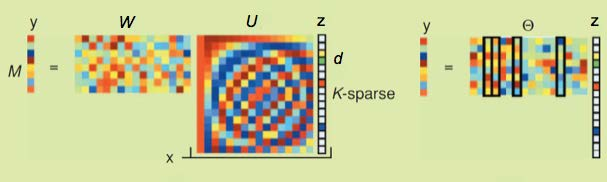
\includegraphics[width=10cm]{fig_10_1.jpg} 
	\caption{A visualization of the idea behind compressive sensing.}\label{fig_10_1}
\end{figure}
\par One might ask, under what condition will it be possible to reconstruct the signal ${\bf x}$ (equivalent to require reconstruction for ${\bf z}$ since given ${\bf U}$ we have ${\bf x}={\bf Uz}$). Surprisingly given any orthonormal basis ${\bf U}$ we can obtain a stable reconstruction for any $K$-sparse compressible signal, if we choose ${\bf W}$ to be a Gaussian random projection, i.e. $w_{ij}\sim \mathcal{N}(0,\frac{1}{D})$ with $M\geq cK\log(\frac{D}{K})$, where $c$ is some constant. Note that the dimension $D$ has only log effects.
\begin{remark}
	Since ${\bf U}$ is an orthonormal matrix, ${\bf \Theta}={\bf WU}$ will remain a Gaussian random projection. It can be shown that there exists a constant $c$ such that if
	\begin{equation*}
		M\geq cK\log(\frac{D}{K}),
	\end{equation*}
	then ${\bf \Theta}$ (a Gaussian random projection) satisfies the $(K,\frac{1}{3})$-RIP (Definition \ref{def_9_RIP}) with high probability. Then with theorem \ref{thm_9_RIP}, we can reconstruct any sparse vector by solving the $L_1$ minimizing problem:
	\begin{equation*}
		\min \|{\bf z}\|_1,\ {\rm s.t.}\ {\bf y}={\bf \Theta z}.
	\end{equation*}
\end{remark}
As mentioned, recovering ${\bf x}$ is equivalent to find ${\bf z}$ which is $K$-sparse. Again we see it is an ill-posed problem since there are more unknowns than equations ($M\ll D$). Note that here the problem does not raise from the overcompleteness but from the sensing matrix by design. We can again require constraints on sparseness to make it a proper optimization problem, where we try to solve
\begin{equation*}
	{\bf z}^*\in \mathop{\arg\min}_{\bf z}\|{\bf z}\|_0,\ \text{s.t. }{\bf y}={\bf \Theta z}.
\end{equation*} 
We can apply the same reconstruction techniques as before: (1) convex optimization (use a surrogate $\|\cdot\|_1$ instead) or (2) Matching Pursuit.
\section{Dictionary Learning}
Now let's move on to the topic of dictionary learning. In all previous cases including compressive sensing, we always assume the transform matrix ${\bf U}$ is known. But can we work with better and more problem specific dictionaries? Recall the fixed orthonormal basis setting:
\begin{equation*}
	{\bf x} = \underbrace{U}_{D\times D}\cdot {\bf z},
\end{equation*}
where we benefit from the efficient inversion of ${\bf U}$: ${\bf z} = {\bf U}^T{\bf x}$, while as a strong priori assumption one ${\bf U}$ usually only works for specific classes of signals; for the oversampling basis setting:
\begin{equation*}
{\bf x} = \underbrace{U}_{D\times L}\cdot {\bf z},\ L>D,
\end{equation*}
we can have sparse coding for several signal classes (or classes with mixture of characteristics), but finding such the sparsest coding may require approximation algorithms (e.g. matching pursuit) and can be problematic if dictionary size $L$ and coherence $m(\bf U)$ are large. The advantage of learning is that we can adapt a dictionary to signal characteristics of the given data set resulting in the same approximation error achievable with smaller $L$.
\subsection{Basic Idea}
To learn a dictionary, first assume we are given a set of images/data (data set).  The idea is to write the transform in a matrix form giving the following matrix factorization problem
\begin{equation}
	\underbrace{\bf X}_{D\times N}\approx \underbrace{\bf U}_{D\times L}\cdot \underbrace{\bf Z}_{L\times N},
\end{equation} 
where ${\bf X}=[{\bf x}_1,\dots,{\bf x}_N]$ is the data matrix, ${\bf U}=[{\bf u}_1,\dots,{\bf u}_L]$ is the dictionary matrix, and ${\bf Z}=[{\bf z}_1,\dots,{\bf z}_N]$. As a dictionary learning problem, we also require constrains further constraints on:
\begin{itemize}
	\item ${\bf U}$: columns/atoms are norm-normalized
	\item ${\bf Z}$: the coding ${\bf z}_i$ should be sparse.
\end{itemize}
Before we move to how we can solve this rather scaring problem, let's first take a look at how can we banefit from this adaptive dictionary. Figure \ref{fig_10_2} shows an example of dictionary learning for $8\times 8$ pixel image patches of face images. We see that the learned dictionary looks quite different from the fixed ones in the sense of randomness. However, they share some similarities as in the learned dictionary there are many atoms seems like edge detectors (but in some different directions).
\begin{figure}[h] 
	\centering 
	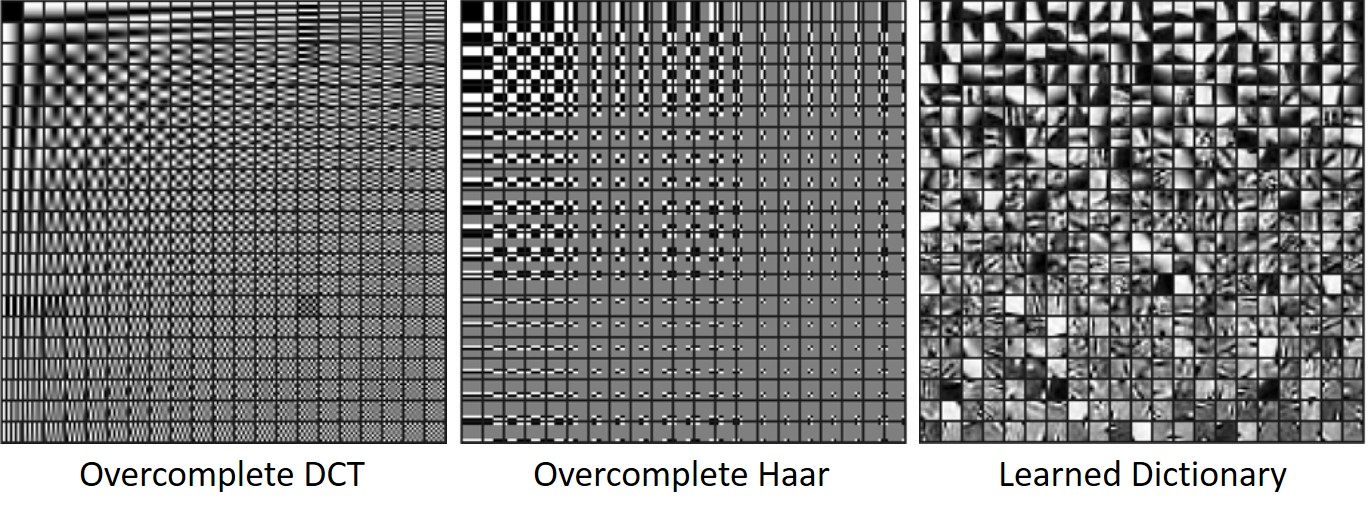
\includegraphics[width=10cm]{fig_10_2.jpg} 
	\caption{Example of dictionary learning from M. Aharon et al. 2006}\label{fig_10_2}
\end{figure}
\par Dictionary learning can also be used for image inpainting, where we are given an image with a mask indicating where it is missing, and we need to complete the image. The idea is really that, a dictionary will do better in inpainting if it's more adapted to the signal. We can construct a sparse coding of observed pixels and predict missing pixels from the sparse code (in some sense similar to denoising).
\begin{figure}[h] 
	\centering 
	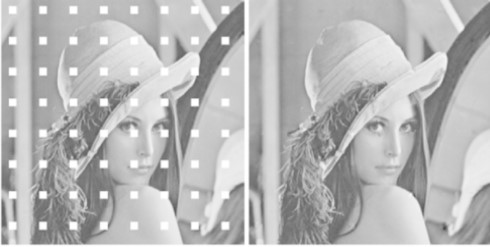
\includegraphics[width=8cm]{fig_10_3.jpg} 
	\caption{Image inpainting (from the internet).}\label{fig_10_3}
\end{figure}
\subsection{Matrix Factorization and K-SVD}
Formally speaking, learning a dictionary with corresponding coding for a given data set ${\bf X}$ is to solve the following matrix factorization problem
\begin{equation*}
	({\bf U^*,Z^*})\in \mathop{\arg\min}_{{\bf U,Z}}\|{\bf X}-UZ\|^2_F,
\end{equation*}
where $\|\cdot\|_F$ is the Frobenius norm defined by $\|{\bf A}\|_F^2=\sum_{i,j}a_{ij}^2$. The hardness comes from that the objective is not jointly convex in ${\bf U}$ and ${\bf Z}$, and different from the situation we have faced, it is not even convex in either ${\bf U}$ and ${\bf Z}$ given that the columns of ${\bf Z}$ are sparse and atoms of ${\bf U}$ are normalized. Still, we can try a iterative greedy minimization:
\begin{enumerate}
	\item \textbf{Coding step:} With fixed dictionary ${\bf U}$ we update the coding matrix via
	\begin{equation}\label{eq_10_obj_coding}
		{\bf Z}^{t+1}\in \mathop{\arg\min}_{\bf Z} \|{\bf X}-{\bf U}^t{\bf Z}\|_F^2,
	\end{equation}
	subject to ${\bf Z}$ being sparse (non-convex constraint).
	\item \textbf{Dictionary update step:} We update the dictionary via
	\begin{equation}\label{eq_10_obj_dic}
		{\bf U}^{t+1}\in \mathop{\arg\min}_{\bf U} \|{\bf X}-{\bf U}{\bf Z}^{t+1}\|_F^2,
	\end{equation}
	subject to $\|{\bf u}_l\|_2=1$ for all $l=1,\dots,L$ (non-convex either) and ${\bf Z}$ being fixed (actually we will update ${\bf Z}$ at the same time in K-SVD).
\end{enumerate}
Let's first discuss the coding step, then continue with the dictionary update and K-SVD.
\par As the first step, we use column separable property of Frobenius norm
\begin{equation*}
	\|{\bf R}\|^2_F = \sum_{i,j}r_{i,j}^2 = \sum_j \|{\bf r}_j\|_2^2
\end{equation*}
to rewrite the objective in (\ref{eq_10_obj_coding}) into
\begin{equation*}
	\sum_{n=1}^N\|{\bf x}_n-{\bf U}^t {\bf z}_n\|_2^2.
\end{equation*}
This means that given ${\bf U}^t$ fixed  we can optimize the columns of ${\bf Z}$ separately meaning we can have $N$ independent sparse coding steps for all $n=1,\dots,N$:
\begin{equation*}
	{\bf z}_n^{t+1}\in \mathop{\arg\min}_{\bf z}\|{\bf x}_n-{\bf U}^t {\bf z}\|_2,
\end{equation*}
where ${\bf z}_n^{t+1}$ needs to be sparse. Instead of solving this problem directly, we can consider a similar problem, where we maximize the sparsity under some tolerance reconstruction error:
\begin{equation}\label{eq_10_coding_pblm}
	{\bf z}_n^{t+1} \in \mathop{\arg\min}_{\bf z} \|{\bf z}\|_0,\quad \text{s.t. }\|{\bf x}_n-{\bf U}^t {\bf z}\|_2\leq \sigma\cdot \|{\bf x}_n\|_2.
\end{equation}
Here $\sigma$ is a tolerance factor, which means instead of requiring exact recovery, we loosen the constraint a little bit for not being too aggressive in one step. The norm of ${\bf x}_n$ in the constraint is because we want to let our tolerance factor invarient to rescaling (multiplying a constant to all data vector). 
\par The two problem is closely related via \textbf{duality}. The following discussion gives some insight on how can these two problem relate to each other. Consider the following two optimization problems:
\begin{align}
	\label{eq_10_p1}&\min_x f(x)\ {\rm s.t.}\ g(x)\leq s\\
	\label{eq_10_p2}&\min_x g(x)\ {\rm s.t.}\ f(x)\leq t,
\end{align}
where $f$ and $g$ are some functions. For example, $f({\bf z}) = \|{\bf x}_n-{\bf U}^t {\bf z}\|_2$ and $g({\bf z}) = \|{\bf z}\|_0$ recover our setting if we formalize the sparse constraint on ${\bf z}$ as being $s$-sparse.
The Lagrangian of (\ref{eq_10_p1}) gives
\begin{equation*}
	L_1 = f(x)+\lambda_1(g(x)-s),
\end{equation*}
and the first-order optimality condition yields:
\begin{equation}\label{eq_10_1st_od_p1}
	\frac{\partial L_1}{\partial x}=f'(x)+\lambda_1g'(x)=0\Rightarrow f'(x)=-\lambda_1g'(x).
\end{equation}
Now do the same for the second problem:
\begin{align}
	&L_2 = g(x)+\lambda_2(f(x)-r)\notag \\
	\label{eq_10_1st_od_p2}&\frac{\partial L_2}{\partial x}=g'(x)+\lambda_2f'(x)=0\Rightarrow g'(x)=-\lambda_2f'(x).
\end{align}
We see that if $\lambda_1=\frac{1}{\lambda_2}$, (\ref{eq_10_1st_od_p1}) and (\ref{eq_10_1st_od_p2}) are the same and the two problem becomes equivalent. 
\par Assume that we can update the coding matrix via \ref{eq_10_coding_pblm}, the next to do is to determine the update rule for the dictionary. Recall the objective for dictionary updating:
\begin{equation*}
	{\bf U}^{t+1}\in \mathop{\arg\min}_{\bf U} \|{\bf X}-{\bf U}{\bf Z}^{t+1}\|_F^2,\ {\rm s.t. }\ \|{\bf u}_l\|_2=1\ \forall l=1,\dots,L.
\end{equation*}
The residual is no longer separable in atoms (columns of ${\bf U}$). This agrees with the observation that the choice of one atom can affect the others at least in this learning setting. The idea is then to update one atom at a time: for all $l$:
\begin{enumerate}
	\item set ${\bf U}=[{\bf u}_1^t\cdots {\bf u}_l^t\cdots {\bf u}_L^t]$, i.e. fix all atoms except ${\bf u}_l$;
	\item isolate/compute ${\bf R}_l^t$, the residual that is independent from atom ${\bf u}_l$;
	\item find ${\bf u}_l^*$ that minimizes ${\bf R}_l^t$ subject to $\|{\bf u}_l^*\|_2=1$.
\end{enumerate}
Formally, in the first and the second step, we compute
\begin{align}
	&\|{\bf X}-[{\bf u}_1^t\cdots {\bf u}_l^t\cdots {\bf u}_L^t]\cdot {\bf Z}^{t+1}\|_F^2\notag\\
	=&\left\|{\bf X}-\left(\sum_{n\neq l}{\bf u}_n^t({\bf z}_n^{t+1})^T + {\bf u}_l^t({\bf z}_l^{t+1})^T\right)\right\|_F^2\notag\\
	\label{eq_10_dic_SVD_obj}=&\left\|{\bf R}_l^t-{\bf u}_l^t({\bf z}_l^{t+1})^T\right\|_F^2,
\end{align}
where ${\bf z}_n^T$ is the $n$-th row of ${\bf Z}$. Note that it's not clear if a specific row of ${\bf Z}$ is sparse (consider that there are some ``popular'' atoms). From (\ref{eq_10_dic_SVD_obj}) we see again we fall into a matrix factorization problem, where we are approximating ${\bf R}_l^t$ with some rank-1 matrix ${\bf u}_l^t({\bf z}_l^{t+1})^T$. The optimal solution is given by SVD of ${\bf R}_l^t$:
\begin{equation*}
	{\bf R}_l^t=\tilde{\bf U}{\bf \Sigma}\tilde{\bf V}=\sum_i \sigma_i \tilde{\bf u}_i\tilde{\bf v}_i^T,\ {\bf u}_l^*=\tilde{\bf u}_1,\ ({\bf z}_l^{*})^T = \sigma_1\tilde{\bf v}_1^T,
\end{equation*}
where we see $\|{\bf u}_l^*\|_2=1$ is naturally satisfied. Recall that in the greedy setting, we are going to update ${\bf U}$ with fixed ${\bf Z}$. However, as suggested by K-SVD, it better not to be too greedy, i.e. we also update the $l$-th row of ${\bf Z}$ with $({\bf z}_l^{*})^T = \sigma_i\tilde{\bf v}_1^T$. One reason for this is that being too greedy will stuck the learning process at local minimums, and another is from that the atom determined by SVD also gives some insight about a good code under ${\bf u}_l^*$. This update is known as approximate K-SVD dictionary update. The name suggests some similarities with K-means algorithm, where in K-means we update $K$ cluster centers with the mean of points assigned to it, while in K-SVD we update K (or L in our notation) atoms with SVD. The actual K-SVD update is a little bit different from the things we have discussed. Let's first look at the algorithm:
\begin{algorithm}
	\caption{Approximate K-SVD Dictionary Update}
	\begin{algorithmic}[1]
		\Require ${\bf X}\in \mathbb{R}^{D\times N}$; ${\bf U}\in \mathbb{R}^{D\times L}; {\bf Z}\in \mathbb{R}^{L\times N}$
		\Ensure Updated dictionary ${\bf U}$
		\For{$l\leftarrow 1$ to $L$}
			\State ${\bf U}_{(:,l)}\leftarrow {\bf 0}$ \Comment{Set the $l$-th atom to zero for isolating ${\bf R}$.}
			\State $\mathcal{N}\leftarrow\{n|Z_{ln}\neq0,1\leq n\neq N\}$ \Comment{Update only active data points.}
			\State ${\bf R}\leftarrow{\bf X}_{(:,\mathcal{N})}-{\bf UZ}_{(:,\mathcal{N})}$	\Comment{Residual independent to the $l$-th atom.}
			\State ${\bf g}\leftarrow {\bf z}^T_{l,\mathcal{N}}$
			\State ${\bf h}\leftarrow {\bf Rg}/\|{\bf Rg}\|$ \Comment{One single step of power iteration.}
			\State ${\bf g}\leftarrow {\bf R}^T{\bf h}$	\Comment{If ${\bf h}=\tilde{\bf u}_1$, ${\bf g}$ will be $ \sigma_1\tilde{\bf v}_1$}
			\State ${\bf U}_{(:,l)}\leftarrow {\bf h}$ \Comment{Update atom.}
			\State ${\bf z}^T_{l,\mathcal{N}}\leftarrow {\bf g}^T$ \Comment{Update corresponding row of ${\bf Z}$}
		\EndFor
	\end{algorithmic}
\end{algorithm}
\par As we can see there are many engineering tricks involved in the algorithm. The updating is restricted to elements (columns) whose coding for the $l$-th atom is non-zero. This has three immediate effects: 
\begin{itemize}
	\item It's computationally efficient.
	\item The sparsity of ${\bf Z}$ will not decrease in the dictionary update step since no entry of ${\bf Z}$ that originally is $0$ will be set to non-zero (we only update ${\bf Z}$ where it's non-zero). Recall that in the coding step, we minimize the $L_0$ norm for columns of ${\bf Z}$, hence the sparsity of ${\bf Z}$ increases in the steps.
	\item The residual ${\bf R}$ is different from ${\bf R}_l^t$ as we have discussed before, where ${\bf R}$ is a sub-matrix of ${\bf R}_l^t$, so SVD will give different results.
\end{itemize} 
The power iteration in line 6 is only performed once, which is also totally an engineering choice. The one might found, the update is order-dependent, i.e. updating with a different order of atoms will give a different result. There is no theoretical guarantees for the output results. The algorithm is also sensitive to the choice of ${\bf U}^0$, with which we optimize locally and greedily until no progress possible. The following are some typical choices for initialization:
\begin{enumerate}[A)]
	\item \textbf{Random atoms}: Sampling ${\bf u}_l^0$ on the unit sphere. This can be done by utilizing the isotropy of Gaussian:
	\begin{enumerate}[1.]
		\item Sample with standard normal distribution: ${\bf u}_l^0\sim \mathcal{N}(0,{\bf I}_D)$.
		\item Scale to unit length: ${\bf u}_l^0\leftarrow {\bf u}_l^0/\|{\bf u}_l^0\|_2$.
	\end{enumerate}
	\item \textbf{Samples from} ${\bf X}$:
	\begin{enumerate}[1.]
		\item ${\bf u}_l^0\leftarrow {\bf x}_n$, where $n\sim \mathcal{U}(1,N)$ is sampled uniformly.
		\item Scale to unit length: ${\bf u}_l^0\leftarrow {\bf u}_l^0/\|{\bf u}_l^0\|_2$.
	\end{enumerate}
	\item \textbf{Fixed overcomplete dictionary:} e.g. use overcomplete DCT.
\end{enumerate}
\par The sildes end with some example which is rather tedious to put here, so we just end here. Thanks for reading and have a nice day:)

\end{document}
